\documentclass[twoside]{book}

% Packages required by doxygen
\usepackage{fixltx2e}
\usepackage{calc}
\usepackage{doxygen}
\usepackage[export]{adjustbox} % also loads graphicx
\usepackage{graphicx}
\usepackage[utf8]{inputenc}
\usepackage{makeidx}
\usepackage{multicol}
\usepackage{multirow}
\PassOptionsToPackage{warn}{textcomp}
\usepackage{textcomp}
\usepackage[nointegrals]{wasysym}
\usepackage[table]{xcolor}

% Font selection
\usepackage[T1]{fontenc}
\usepackage[scaled=.90]{helvet}
\usepackage{courier}
\usepackage{amssymb}
\usepackage{sectsty}
\renewcommand{\familydefault}{\sfdefault}
\allsectionsfont{%
  \fontseries{bc}\selectfont%
  \color{darkgray}%
}
\renewcommand{\DoxyLabelFont}{%
  \fontseries{bc}\selectfont%
  \color{darkgray}%
}
\newcommand{\+}{\discretionary{\mbox{\scriptsize$\hookleftarrow$}}{}{}}

% Page & text layout
\usepackage{geometry}
\geometry{%
  a4paper,%
  top=2.5cm,%
  bottom=2.5cm,%
  left=2.5cm,%
  right=2.5cm%
}
\tolerance=750
\hfuzz=15pt
\hbadness=750
\setlength{\emergencystretch}{15pt}
\setlength{\parindent}{0cm}
\setlength{\parskip}{3ex plus 2ex minus 2ex}
\makeatletter
\renewcommand{\paragraph}{%
  \@startsection{paragraph}{4}{0ex}{-1.0ex}{1.0ex}{%
    \normalfont\normalsize\bfseries\SS@parafont%
  }%
}
\renewcommand{\subparagraph}{%
  \@startsection{subparagraph}{5}{0ex}{-1.0ex}{1.0ex}{%
    \normalfont\normalsize\bfseries\SS@subparafont%
  }%
}
\makeatother

% Headers & footers
\usepackage{fancyhdr}
\pagestyle{fancyplain}
\fancyhead[LE]{\fancyplain{}{\bfseries\thepage}}
\fancyhead[CE]{\fancyplain{}{}}
\fancyhead[RE]{\fancyplain{}{\bfseries\leftmark}}
\fancyhead[LO]{\fancyplain{}{\bfseries\rightmark}}
\fancyhead[CO]{\fancyplain{}{}}
\fancyhead[RO]{\fancyplain{}{\bfseries\thepage}}
\fancyfoot[LE]{\fancyplain{}{}}
\fancyfoot[CE]{\fancyplain{}{}}
\fancyfoot[RE]{\fancyplain{}{\bfseries\scriptsize Generated by Doxygen }}
\fancyfoot[LO]{\fancyplain{}{\bfseries\scriptsize Generated by Doxygen }}
\fancyfoot[CO]{\fancyplain{}{}}
\fancyfoot[RO]{\fancyplain{}{}}
\renewcommand{\footrulewidth}{0.4pt}
\renewcommand{\chaptermark}[1]{%
  \markboth{#1}{}%
}
\renewcommand{\sectionmark}[1]{%
  \markright{\thesection\ #1}%
}

% Indices & bibliography
\usepackage{natbib}
\usepackage[titles]{tocloft}
\setcounter{tocdepth}{3}
\setcounter{secnumdepth}{5}
\makeindex

% Hyperlinks (required, but should be loaded last)
\usepackage{ifpdf}
\ifpdf
  \usepackage[pdftex,pagebackref=true]{hyperref}
\else
  \usepackage[ps2pdf,pagebackref=true]{hyperref}
\fi
\hypersetup{%
  colorlinks=true,%
  linkcolor=blue,%
  citecolor=blue,%
  unicode%
}

% Custom commands
\newcommand{\clearemptydoublepage}{%
  \newpage{\pagestyle{empty}\cleardoublepage}%
}

\usepackage{caption}
\captionsetup{labelsep=space,justification=centering,font={bf},singlelinecheck=off,skip=4pt,position=top}

%===== C O N T E N T S =====

\begin{document}

% Titlepage & ToC
\hypersetup{pageanchor=false,
             bookmarksnumbered=true,
             pdfencoding=unicode
            }
\pagenumbering{alph}
\begin{titlepage}
\vspace*{7cm}
\begin{center}%
{\Large My Project }\\
\vspace*{1cm}
{\large Generated by Doxygen 1.8.14}\\
\end{center}
\end{titlepage}
\clearemptydoublepage
\pagenumbering{roman}
\tableofcontents
\clearemptydoublepage
\pagenumbering{arabic}
\hypersetup{pageanchor=true}

%--- Begin generated contents ---
\chapter{R\+E\+A\+D\+ME}
\label{md_README}
\Hypertarget{md_README}
Copy this entire folder to be under your hw7 folder (i.\+e. it should be at hw-\/username/hw7/hw7-\/check).

Run {\ttfamily make compile\+\_\+check} to check whether each class compiles. There are four compilation tests and you need to pass all of them.

Run {\ttfamily make test} to check if your \mbox{\hyperlink{classBinarySearchTree}{Binary\+Search\+Tree}} and rotate\+B\+ST pass the basic functionality tests. You should pass both G\+T\+E\+S\+Ts.

Run {\ttfamily make hypercube\+\_\+test} to check if you hypercube pass the basic functionality tests. You can find the start node for each test in {\ttfamily hw7-\/check/start.\+txt}, permitted nodes in {\ttfamily hw7-\/check/permitted$<$X$>$.txt}, and expected output in {\ttfamily hw7-\/check/solution$<$X$>$.txt}.

Passing all compilation and functionality tests is not a guarantee of your score. However, failing any of the tests means you will likely lose significant points on the homework. 
\chapter{Hierarchical Index}
\section{Class Hierarchy}
This inheritance list is sorted roughly, but not completely, alphabetically\+:\begin{DoxyCompactList}
\item \contentsline{section}{Binary\+Search\+Tree$<$ Key, Value $>$}{\pageref{classBinarySearchTree}}{}
\begin{DoxyCompactList}
\item \contentsline{section}{Inherited\+B\+ST$<$ Key, Value $>$}{\pageref{classInheritedBST}}{}
\item \contentsline{section}{Inherited\+B\+ST$<$ Key, Value $>$}{\pageref{classInheritedBST}}{}
\end{DoxyCompactList}
\item \contentsline{section}{Binary\+Search\+Tree$<$ Key, Value $>$\+:\+:iterator}{\pageref{classBinarySearchTree_1_1iterator}}{}
\item \contentsline{section}{Node$<$ Key, Value $>$}{\pageref{classNode}}{}
\begin{DoxyCompactList}
\item \contentsline{section}{Inherited\+Node$<$ Key, Value $>$}{\pageref{classInheritedNode}}{}
\end{DoxyCompactList}
\item rotate\+B\+ST\begin{DoxyCompactList}
\item \contentsline{section}{Inherited\+Rotate$<$ Key, Value $>$}{\pageref{classInheritedRotate}}{}
\item \contentsline{section}{Inherited\+Rotate$<$ Key, Value $>$}{\pageref{classInheritedRotate}}{}
\end{DoxyCompactList}
\item Test\begin{DoxyCompactList}
\item \contentsline{section}{B\+S\+T\+Test}{\pageref{classBSTTest}}{}
\item \contentsline{section}{Rotate\+Test}{\pageref{classRotateTest}}{}
\end{DoxyCompactList}
\end{DoxyCompactList}

\chapter{Class Index}
\section{Class List}
Here are the classes, structs, unions and interfaces with brief descriptions\+:\begin{DoxyCompactList}
\item\contentsline{section}{\mbox{\hyperlink{classBinarySearchTree}{Binary\+Search\+Tree$<$ Key, Value $>$}} }{\pageref{classBinarySearchTree}}{}
\item\contentsline{section}{\mbox{\hyperlink{classBSTTest}{B\+S\+T\+Test}} }{\pageref{classBSTTest}}{}
\item\contentsline{section}{\mbox{\hyperlink{classInheritedBST}{Inherited\+B\+S\+T$<$ Key, Value $>$}} }{\pageref{classInheritedBST}}{}
\item\contentsline{section}{\mbox{\hyperlink{classInheritedNode}{Inherited\+Node$<$ Key, Value $>$}} }{\pageref{classInheritedNode}}{}
\item\contentsline{section}{\mbox{\hyperlink{classInheritedRotate}{Inherited\+Rotate$<$ Key, Value $>$}} }{\pageref{classInheritedRotate}}{}
\item\contentsline{section}{\mbox{\hyperlink{classBinarySearchTree_1_1iterator}{Binary\+Search\+Tree$<$ Key, Value $>$\+::iterator}} }{\pageref{classBinarySearchTree_1_1iterator}}{}
\item\contentsline{section}{\mbox{\hyperlink{classNode}{Node$<$ Key, Value $>$}} }{\pageref{classNode}}{}
\item\contentsline{section}{\mbox{\hyperlink{classRotateTest}{Rotate\+Test}} }{\pageref{classRotateTest}}{}
\end{DoxyCompactList}

\chapter{Class Documentation}
\hypertarget{classBinarySearchTree}{}\section{Binary\+Search\+Tree$<$ Key, Value $>$ Class Template Reference}
\label{classBinarySearchTree}\index{Binary\+Search\+Tree$<$ Key, Value $>$@{Binary\+Search\+Tree$<$ Key, Value $>$}}


{\ttfamily \#include $<$hw7\+\_\+provided\+\_\+bst.\+h$>$}

Inheritance diagram for Binary\+Search\+Tree$<$ Key, Value $>$\+:\begin{figure}[H]
\begin{center}
\leavevmode
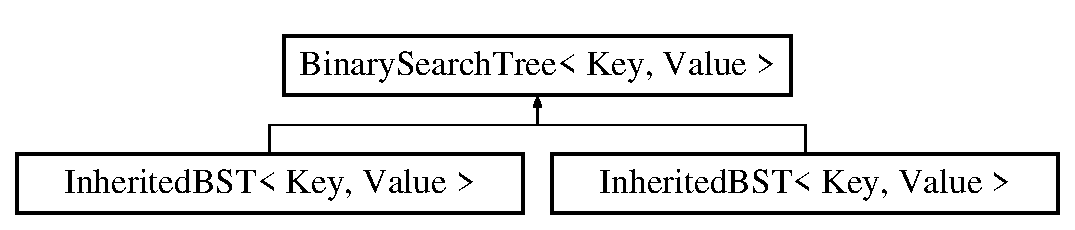
\includegraphics[height=2.000000cm]{classBinarySearchTree}
\end{center}
\end{figure}
\subsection*{Classes}
\begin{DoxyCompactItemize}
\item 
class \mbox{\hyperlink{classBinarySearchTree_1_1iterator}{iterator}}
\end{DoxyCompactItemize}
\subsection*{Public Member Functions}
\begin{DoxyCompactItemize}
\item 
\mbox{\hyperlink{classBinarySearchTree_ad755ed0485364094f462ce45cf6ecf62}{Binary\+Search\+Tree}} ()
\item 
int \mbox{\hyperlink{classBinarySearchTree_af3cd6ac851903ea24fb3be48f10c4015}{height}} ()
\item 
bool \mbox{\hyperlink{classBinarySearchTree_afd462b85819b2ed73bde24c3383b673b}{is\+Balanced}} ()
\item 
virtual void \mbox{\hyperlink{classBinarySearchTree_a20c129156570a782fe10b1d803928a4c}{insert}} (const std\+::pair$<$ const Key, Value $>$ \&key\+Value\+Pair)
\item 
virtual void \mbox{\hyperlink{classBinarySearchTree_a23a65055a8e1d1f501f89140c219bda2}{remove}} (const Key \&key)
\item 
void \mbox{\hyperlink{classBinarySearchTree_acce1030d8eb99522591b90e0824e7bbc}{clear}} ()
\item 
\mbox{\Hypertarget{classBinarySearchTree_acaffd92012c913f3a04a75dd6d07d488}\label{classBinarySearchTree_acaffd92012c913f3a04a75dd6d07d488}} 
void {\bfseries print} () const
\item 
\mbox{\hyperlink{classBinarySearchTree_1_1iterator}{iterator}} \mbox{\hyperlink{classBinarySearchTree_ac42b6e11e290cf9eaf56eba56ca56818}{begin}} ()
\item 
\mbox{\hyperlink{classBinarySearchTree_1_1iterator}{iterator}} \mbox{\hyperlink{classBinarySearchTree_a6603b43057a4bf2843381b8abcb0d010}{end}} ()
\item 
\mbox{\hyperlink{classBinarySearchTree_1_1iterator}{iterator}} \mbox{\hyperlink{classBinarySearchTree_ad8772cfce540ec1d9279c674bdb01e40}{find}} (const Key \&key) const
\end{DoxyCompactItemize}
\subsection*{Protected Member Functions}
\begin{DoxyCompactItemize}
\item 
\mbox{\hyperlink{classNode}{Node}}$<$ Key, Value $>$ $\ast$ \mbox{\hyperlink{classBinarySearchTree_aed5147cde1f6bb15aa192456b7a1f20c}{internal\+Find}} (const Key \&key) const
\item 
\mbox{\hyperlink{classNode}{Node}}$<$ Key, Value $>$ $\ast$ \mbox{\hyperlink{classBinarySearchTree_a04d73a5c985288b8837c2629c3ee0e39}{get\+Smallest\+Node}} () const
\item 
void \mbox{\hyperlink{classBinarySearchTree_a6996f52ecfb5a0d1f62432a7b3b792b5}{print\+Root}} (\mbox{\hyperlink{classNode}{Node}}$<$ Key, Value $>$ $\ast$root) const
\end{DoxyCompactItemize}
\subsection*{Protected Attributes}
\begin{DoxyCompactItemize}
\item 
\mbox{\Hypertarget{classBinarySearchTree_a86747f59a7d863080da23a74bea8ed1c}\label{classBinarySearchTree_a86747f59a7d863080da23a74bea8ed1c}} 
\mbox{\hyperlink{classNode}{Node}}$<$ Key, Value $>$ $\ast$ {\bfseries m\+Root}
\end{DoxyCompactItemize}


\subsection{Detailed Description}
\subsubsection*{template$<$typename Key, typename Value$>$\newline
class Binary\+Search\+Tree$<$ Key, Value $>$}

A templated unbalanced binary search tree. 

\subsection{Constructor \& Destructor Documentation}
\mbox{\Hypertarget{classBinarySearchTree_ad755ed0485364094f462ce45cf6ecf62}\label{classBinarySearchTree_ad755ed0485364094f462ce45cf6ecf62}} 
\index{Binary\+Search\+Tree@{Binary\+Search\+Tree}!Binary\+Search\+Tree@{Binary\+Search\+Tree}}
\index{Binary\+Search\+Tree@{Binary\+Search\+Tree}!Binary\+Search\+Tree@{Binary\+Search\+Tree}}
\subsubsection{\texorpdfstring{Binary\+Search\+Tree()}{BinarySearchTree()}}
{\footnotesize\ttfamily template$<$typename Key , typename Value $>$ \\
\mbox{\hyperlink{classBinarySearchTree}{Binary\+Search\+Tree}}$<$ Key, Value $>$\+::\mbox{\hyperlink{classBinarySearchTree}{Binary\+Search\+Tree}} (\begin{DoxyParamCaption}{ }\end{DoxyParamCaption})}

Default constructor for a \mbox{\hyperlink{classBinarySearchTree}{Binary\+Search\+Tree}}, which sets the root to N\+U\+LL. 

\subsection{Member Function Documentation}
\mbox{\Hypertarget{classBinarySearchTree_ac42b6e11e290cf9eaf56eba56ca56818}\label{classBinarySearchTree_ac42b6e11e290cf9eaf56eba56ca56818}} 
\index{Binary\+Search\+Tree@{Binary\+Search\+Tree}!begin@{begin}}
\index{begin@{begin}!Binary\+Search\+Tree@{Binary\+Search\+Tree}}
\subsubsection{\texorpdfstring{begin()}{begin()}}
{\footnotesize\ttfamily template$<$typename Key , typename Value $>$ \\
\mbox{\hyperlink{classBinarySearchTree}{Binary\+Search\+Tree}}$<$ Key, Value $>$\+::\mbox{\hyperlink{classBinarySearchTree_1_1iterator}{iterator}} \mbox{\hyperlink{classBinarySearchTree}{Binary\+Search\+Tree}}$<$ Key, Value $>$\+::begin (\begin{DoxyParamCaption}{ }\end{DoxyParamCaption})}

Returns an iterator to the \char`\"{}smallest\char`\"{} item in the tree \mbox{\Hypertarget{classBinarySearchTree_acce1030d8eb99522591b90e0824e7bbc}\label{classBinarySearchTree_acce1030d8eb99522591b90e0824e7bbc}} 
\index{Binary\+Search\+Tree@{Binary\+Search\+Tree}!clear@{clear}}
\index{clear@{clear}!Binary\+Search\+Tree@{Binary\+Search\+Tree}}
\subsubsection{\texorpdfstring{clear()}{clear()}}
{\footnotesize\ttfamily template$<$typename Key , typename Value $>$ \\
void \mbox{\hyperlink{classBinarySearchTree}{Binary\+Search\+Tree}}$<$ Key, Value $>$\+::clear (\begin{DoxyParamCaption}{ }\end{DoxyParamCaption})}

A method to remove all contents of the tree and reset the values in the tree for use again. \mbox{\Hypertarget{classBinarySearchTree_a6603b43057a4bf2843381b8abcb0d010}\label{classBinarySearchTree_a6603b43057a4bf2843381b8abcb0d010}} 
\index{Binary\+Search\+Tree@{Binary\+Search\+Tree}!end@{end}}
\index{end@{end}!Binary\+Search\+Tree@{Binary\+Search\+Tree}}
\subsubsection{\texorpdfstring{end()}{end()}}
{\footnotesize\ttfamily template$<$typename Key , typename Value $>$ \\
\mbox{\hyperlink{classBinarySearchTree}{Binary\+Search\+Tree}}$<$ Key, Value $>$\+::\mbox{\hyperlink{classBinarySearchTree_1_1iterator}{iterator}} \mbox{\hyperlink{classBinarySearchTree}{Binary\+Search\+Tree}}$<$ Key, Value $>$\+::end (\begin{DoxyParamCaption}{ }\end{DoxyParamCaption})}

Returns an iterator whose value means I\+N\+V\+A\+L\+ID \mbox{\Hypertarget{classBinarySearchTree_ad8772cfce540ec1d9279c674bdb01e40}\label{classBinarySearchTree_ad8772cfce540ec1d9279c674bdb01e40}} 
\index{Binary\+Search\+Tree@{Binary\+Search\+Tree}!find@{find}}
\index{find@{find}!Binary\+Search\+Tree@{Binary\+Search\+Tree}}
\subsubsection{\texorpdfstring{find()}{find()}}
{\footnotesize\ttfamily template$<$typename Key , typename Value $>$ \\
\mbox{\hyperlink{classBinarySearchTree}{Binary\+Search\+Tree}}$<$ Key, Value $>$\+::\mbox{\hyperlink{classBinarySearchTree_1_1iterator}{iterator}} \mbox{\hyperlink{classBinarySearchTree}{Binary\+Search\+Tree}}$<$ Key, Value $>$\+::find (\begin{DoxyParamCaption}\item[{const Key \&}]{key }\end{DoxyParamCaption}) const}

Returns an iterator to the item with the given key, k or the end iterator if k does not exist in the tree \mbox{\Hypertarget{classBinarySearchTree_a04d73a5c985288b8837c2629c3ee0e39}\label{classBinarySearchTree_a04d73a5c985288b8837c2629c3ee0e39}} 
\index{Binary\+Search\+Tree@{Binary\+Search\+Tree}!get\+Smallest\+Node@{get\+Smallest\+Node}}
\index{get\+Smallest\+Node@{get\+Smallest\+Node}!Binary\+Search\+Tree@{Binary\+Search\+Tree}}
\subsubsection{\texorpdfstring{get\+Smallest\+Node()}{getSmallestNode()}}
{\footnotesize\ttfamily template$<$typename Key , typename Value $>$ \\
\mbox{\hyperlink{classNode}{Node}}$<$ Key, Value $>$ $\ast$ \mbox{\hyperlink{classBinarySearchTree}{Binary\+Search\+Tree}}$<$ Key, Value $>$\+::get\+Smallest\+Node (\begin{DoxyParamCaption}{ }\end{DoxyParamCaption}) const\hspace{0.3cm}{\ttfamily [protected]}}

A helper function to find the smallest node in the tree. \mbox{\Hypertarget{classBinarySearchTree_af3cd6ac851903ea24fb3be48f10c4015}\label{classBinarySearchTree_af3cd6ac851903ea24fb3be48f10c4015}} 
\index{Binary\+Search\+Tree@{Binary\+Search\+Tree}!height@{height}}
\index{height@{height}!Binary\+Search\+Tree@{Binary\+Search\+Tree}}
\subsubsection{\texorpdfstring{height()}{height()}}
{\footnotesize\ttfamily template$<$typename Key , typename Value $>$ \\
int \mbox{\hyperlink{classBinarySearchTree}{Binary\+Search\+Tree}}$<$ Key, Value $>$\+::height (\begin{DoxyParamCaption}{ }\end{DoxyParamCaption})}

An method to return the height of the B\+ST. \mbox{\Hypertarget{classBinarySearchTree_a20c129156570a782fe10b1d803928a4c}\label{classBinarySearchTree_a20c129156570a782fe10b1d803928a4c}} 
\index{Binary\+Search\+Tree@{Binary\+Search\+Tree}!insert@{insert}}
\index{insert@{insert}!Binary\+Search\+Tree@{Binary\+Search\+Tree}}
\subsubsection{\texorpdfstring{insert()}{insert()}}
{\footnotesize\ttfamily template$<$typename Key , typename Value $>$ \\
void \mbox{\hyperlink{classBinarySearchTree}{Binary\+Search\+Tree}}$<$ Key, Value $>$\+::insert (\begin{DoxyParamCaption}\item[{const std\+::pair$<$ const Key, Value $>$ \&}]{key\+Value\+Pair }\end{DoxyParamCaption})\hspace{0.3cm}{\ttfamily [virtual]}}

An insert method to insert into a Binary Search Tree. The tree will not remain balanced when inserting. \mbox{\Hypertarget{classBinarySearchTree_aed5147cde1f6bb15aa192456b7a1f20c}\label{classBinarySearchTree_aed5147cde1f6bb15aa192456b7a1f20c}} 
\index{Binary\+Search\+Tree@{Binary\+Search\+Tree}!internal\+Find@{internal\+Find}}
\index{internal\+Find@{internal\+Find}!Binary\+Search\+Tree@{Binary\+Search\+Tree}}
\subsubsection{\texorpdfstring{internal\+Find()}{internalFind()}}
{\footnotesize\ttfamily template$<$typename Key , typename Value $>$ \\
\mbox{\hyperlink{classNode}{Node}}$<$ Key, Value $>$ $\ast$ \mbox{\hyperlink{classBinarySearchTree}{Binary\+Search\+Tree}}$<$ Key, Value $>$\+::internal\+Find (\begin{DoxyParamCaption}\item[{const Key \&}]{key }\end{DoxyParamCaption}) const\hspace{0.3cm}{\ttfamily [protected]}}

Helper function to find a node with given key, k and return a pointer to it or N\+U\+LL if no item with that key exists \mbox{\Hypertarget{classBinarySearchTree_afd462b85819b2ed73bde24c3383b673b}\label{classBinarySearchTree_afd462b85819b2ed73bde24c3383b673b}} 
\index{Binary\+Search\+Tree@{Binary\+Search\+Tree}!is\+Balanced@{is\+Balanced}}
\index{is\+Balanced@{is\+Balanced}!Binary\+Search\+Tree@{Binary\+Search\+Tree}}
\subsubsection{\texorpdfstring{is\+Balanced()}{isBalanced()}}
{\footnotesize\ttfamily template$<$typename Key , typename Value $>$ \\
bool \mbox{\hyperlink{classBinarySearchTree}{Binary\+Search\+Tree}}$<$ Key, Value $>$\+::is\+Balanced (\begin{DoxyParamCaption}{ }\end{DoxyParamCaption})}

An method to checks if the B\+ST is balanced. This method returns true if and only if the B\+ST is balanced. \mbox{\Hypertarget{classBinarySearchTree_a6996f52ecfb5a0d1f62432a7b3b792b5}\label{classBinarySearchTree_a6996f52ecfb5a0d1f62432a7b3b792b5}} 
\index{Binary\+Search\+Tree@{Binary\+Search\+Tree}!print\+Root@{print\+Root}}
\index{print\+Root@{print\+Root}!Binary\+Search\+Tree@{Binary\+Search\+Tree}}
\subsubsection{\texorpdfstring{print\+Root()}{printRoot()}}
{\footnotesize\ttfamily template$<$typename Key , typename Value $>$ \\
void \mbox{\hyperlink{classBinarySearchTree}{Binary\+Search\+Tree}}$<$ Key, Value $>$\+::print\+Root (\begin{DoxyParamCaption}\item[{\mbox{\hyperlink{classNode}{Node}}$<$ Key, Value $>$ $\ast$}]{root }\end{DoxyParamCaption}) const\hspace{0.3cm}{\ttfamily [protected]}}

Helper function to print the tree\textquotesingle{}s contents \mbox{\Hypertarget{classBinarySearchTree_a23a65055a8e1d1f501f89140c219bda2}\label{classBinarySearchTree_a23a65055a8e1d1f501f89140c219bda2}} 
\index{Binary\+Search\+Tree@{Binary\+Search\+Tree}!remove@{remove}}
\index{remove@{remove}!Binary\+Search\+Tree@{Binary\+Search\+Tree}}
\subsubsection{\texorpdfstring{remove()}{remove()}}
{\footnotesize\ttfamily template$<$typename Key , typename Value $>$ \\
void \mbox{\hyperlink{classBinarySearchTree}{Binary\+Search\+Tree}}$<$ Key, Value $>$\+::remove (\begin{DoxyParamCaption}\item[{const Key \&}]{key }\end{DoxyParamCaption})\hspace{0.3cm}{\ttfamily [virtual]}}

An remove method to remove a specific key from a Binary Search Tree. The tree may not remain balanced after removal. 

The documentation for this class was generated from the following file\+:\begin{DoxyCompactItemize}
\item 
hw7\+\_\+provided\+\_\+bst.\+h\end{DoxyCompactItemize}

\hypertarget{classBSTTest}{}\section{B\+S\+T\+Test Class Reference}
\label{classBSTTest}\index{B\+S\+T\+Test@{B\+S\+T\+Test}}
Inheritance diagram for B\+S\+T\+Test\+:\begin{figure}[H]
\begin{center}
\leavevmode
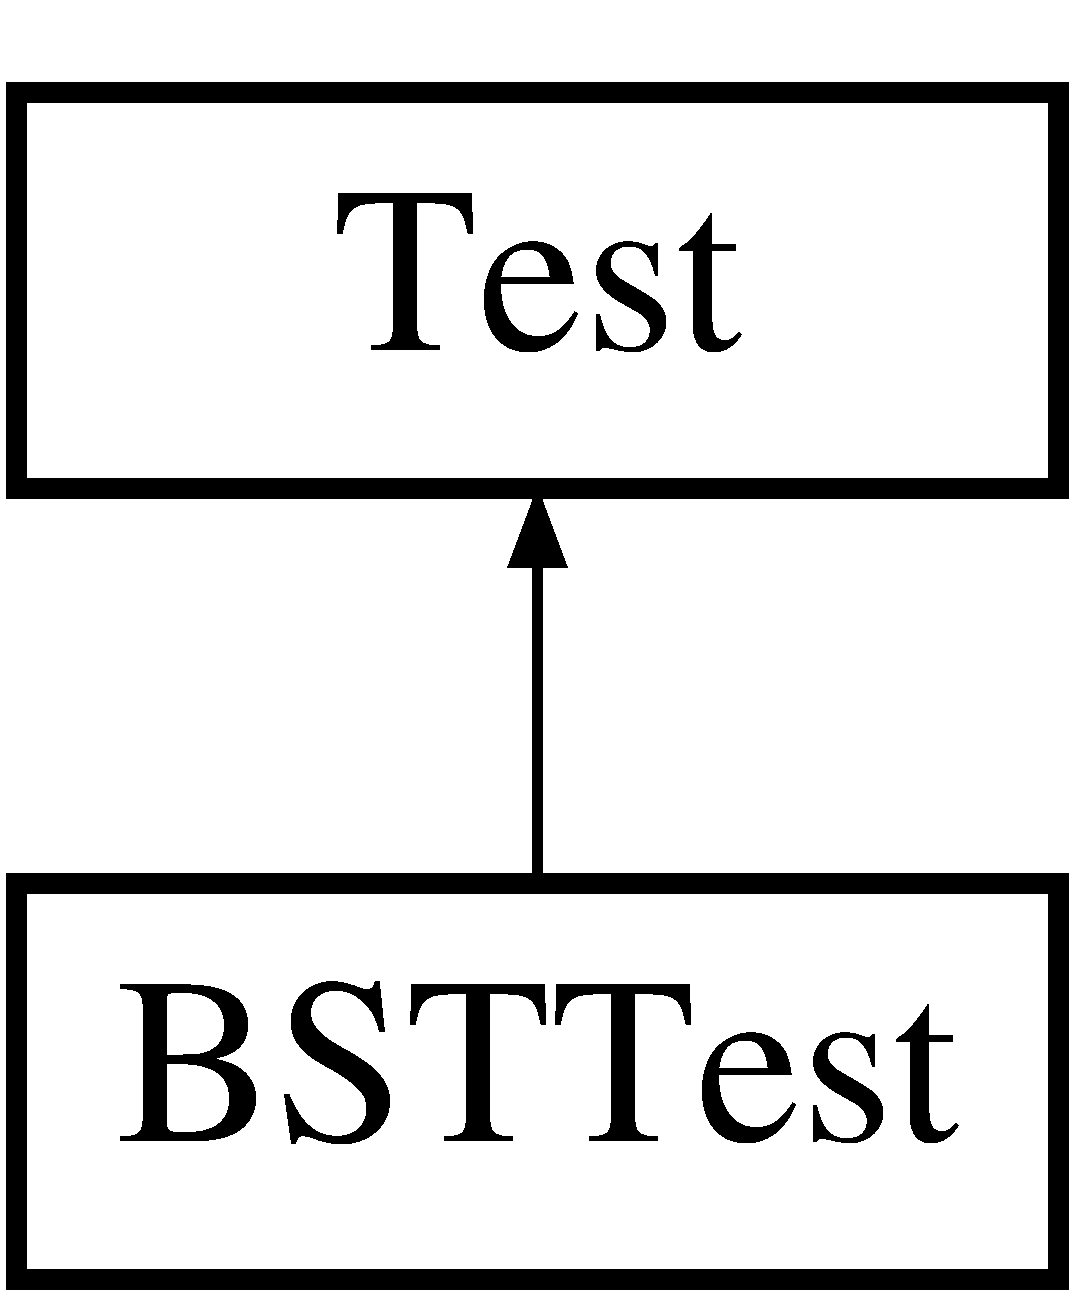
\includegraphics[height=2.000000cm]{classBSTTest}
\end{center}
\end{figure}
\subsection*{Protected Member Functions}
\begin{DoxyCompactItemize}
\item 
\mbox{\Hypertarget{classBSTTest_a04feda0d86547db4b515032b758b3a97}\label{classBSTTest_a04feda0d86547db4b515032b758b3a97}} 
void {\bfseries stress\+Test\+Insert} (size\+\_\+t size, uint seed)
\item 
\mbox{\Hypertarget{classBSTTest_aac738c944fe9607ebe78f02b3343ee6c}\label{classBSTTest_aac738c944fe9607ebe78f02b3343ee6c}} 
void {\bfseries stress\+Test\+Remove} (size\+\_\+t size, uint seed)
\end{DoxyCompactItemize}


The documentation for this class was generated from the following file\+:\begin{DoxyCompactItemize}
\item 
hw7\+\_\+bst\+\_\+test.\+cpp\end{DoxyCompactItemize}

\hypertarget{classInheritedBST}{}\section{Inherited\+B\+ST$<$ Key, Value $>$ Class Template Reference}
\label{classInheritedBST}\index{Inherited\+B\+S\+T$<$ Key, Value $>$@{Inherited\+B\+S\+T$<$ Key, Value $>$}}
Inheritance diagram for Inherited\+B\+ST$<$ Key, Value $>$\+:\begin{figure}[H]
\begin{center}
\leavevmode
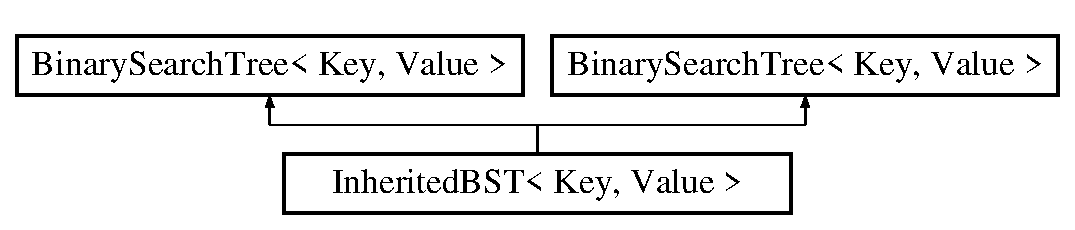
\includegraphics[height=2.000000cm]{classInheritedBST}
\end{center}
\end{figure}
\subsection*{Public Member Functions}
\begin{DoxyCompactItemize}
\item 
\mbox{\Hypertarget{classInheritedBST_a4d08c97a828ea6a3af0a13c29d77250b}\label{classInheritedBST_a4d08c97a828ea6a3af0a13c29d77250b}} 
void {\bfseries test} ()
\item 
\mbox{\Hypertarget{classInheritedBST_a2335cb24692ddfe4b8a140a7b9ba0029}\label{classInheritedBST_a2335cb24692ddfe4b8a140a7b9ba0029}} 
\mbox{\hyperlink{classNode}{Node}}$<$ Key, Value $>$ $\ast$ {\bfseries get\+Root} ()
\end{DoxyCompactItemize}
\subsection*{Additional Inherited Members}


The documentation for this class was generated from the following files\+:\begin{DoxyCompactItemize}
\item 
hw7\+\_\+bst\+\_\+checker.\+cpp\item 
hw7\+\_\+bst\+\_\+test.\+cpp\end{DoxyCompactItemize}

\hypertarget{classInheritedNode}{}\section{Inherited\+Node$<$ Key, Value $>$ Class Template Reference}
\label{classInheritedNode}\index{Inherited\+Node$<$ Key, Value $>$@{Inherited\+Node$<$ Key, Value $>$}}
Inheritance diagram for Inherited\+Node$<$ Key, Value $>$\+:\begin{figure}[H]
\begin{center}
\leavevmode
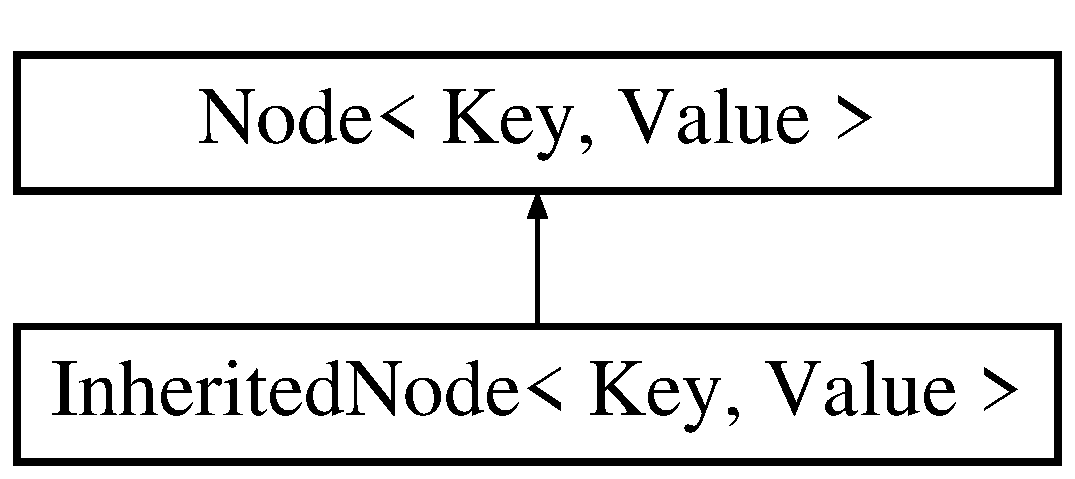
\includegraphics[height=2.000000cm]{classInheritedNode}
\end{center}
\end{figure}
\subsection*{Public Member Functions}
\begin{DoxyCompactItemize}
\item 
\mbox{\Hypertarget{classInheritedNode_aaebcd7037935df516a404688cf1a625a}\label{classInheritedNode_aaebcd7037935df516a404688cf1a625a}} 
{\bfseries Inherited\+Node} (const Key \&key, const Value \&value)
\item 
\mbox{\Hypertarget{classInheritedNode_a33addaefed4aae2c4b2731e57d1fcd1c}\label{classInheritedNode_a33addaefed4aae2c4b2731e57d1fcd1c}} 
void {\bfseries test} ()
\end{DoxyCompactItemize}
\subsection*{Additional Inherited Members}


The documentation for this class was generated from the following file\+:\begin{DoxyCompactItemize}
\item 
hw7\+\_\+node\+\_\+checker.\+cpp\end{DoxyCompactItemize}

\hypertarget{classInheritedRotate}{}\section{Inherited\+Rotate$<$ Key, Value $>$ Class Template Reference}
\label{classInheritedRotate}\index{Inherited\+Rotate$<$ Key, Value $>$@{Inherited\+Rotate$<$ Key, Value $>$}}
Inheritance diagram for Inherited\+Rotate$<$ Key, Value $>$\+:\begin{figure}[H]
\begin{center}
\leavevmode
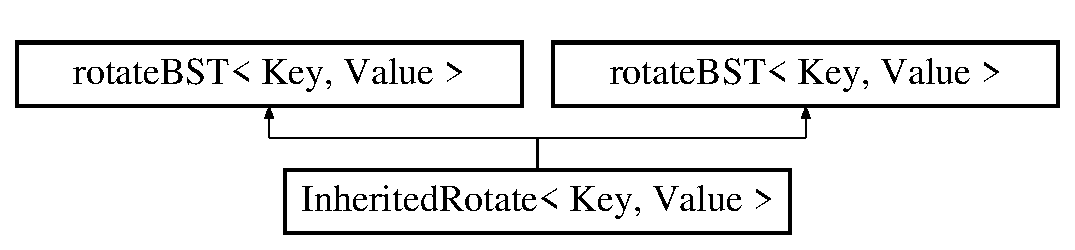
\includegraphics[height=2.000000cm]{classInheritedRotate}
\end{center}
\end{figure}
\subsection*{Public Member Functions}
\begin{DoxyCompactItemize}
\item 
\mbox{\Hypertarget{classInheritedRotate_ac4c24eba0c0dcae88b9784ec504317c7}\label{classInheritedRotate_ac4c24eba0c0dcae88b9784ec504317c7}} 
void {\bfseries test\+Protected\+Members} ()
\item 
\mbox{\Hypertarget{classInheritedRotate_a8d963ec64081e43e592da62cb1a0ac47}\label{classInheritedRotate_a8d963ec64081e43e592da62cb1a0ac47}} 
void {\bfseries test\+Inherited\+Members} ()
\item 
\mbox{\Hypertarget{classInheritedRotate_adec634aab9dba9426e58fc1b619c0eb7}\label{classInheritedRotate_adec634aab9dba9426e58fc1b619c0eb7}} 
void {\bfseries left\+Rotate\+Root} ()
\item 
\mbox{\Hypertarget{classInheritedRotate_a2ea0ef146a955c023df5f314de19a4c5}\label{classInheritedRotate_a2ea0ef146a955c023df5f314de19a4c5}} 
void {\bfseries right\+Rotate\+Root} ()
\item 
\mbox{\Hypertarget{classInheritedRotate_a8719303ced7dd31c3b8370a2f40f54d9}\label{classInheritedRotate_a8719303ced7dd31c3b8370a2f40f54d9}} 
\mbox{\hyperlink{classNode}{Node}}$<$ Key, Value $>$ $\ast$ {\bfseries get\+Root} ()
\end{DoxyCompactItemize}


The documentation for this class was generated from the following files\+:\begin{DoxyCompactItemize}
\item 
hw7\+\_\+rotate\+\_\+checker.\+cpp\item 
hw7\+\_\+rotate\+\_\+test.\+cpp\end{DoxyCompactItemize}

\hypertarget{classBinarySearchTree_1_1iterator}{}\section{Binary\+Search\+Tree$<$ Key, Value $>$\+:\+:iterator Class Reference}
\label{classBinarySearchTree_1_1iterator}\index{Binary\+Search\+Tree$<$ Key, Value $>$\+::iterator@{Binary\+Search\+Tree$<$ Key, Value $>$\+::iterator}}


{\ttfamily \#include $<$hw7\+\_\+provided\+\_\+bst.\+h$>$}

\subsection*{Public Member Functions}
\begin{DoxyCompactItemize}
\item 
\mbox{\hyperlink{classBinarySearchTree_1_1iterator_ad2d047d6e1fda6f9e74a568fd0539d34}{iterator}} (\mbox{\hyperlink{classNode}{Node}}$<$ Key, Value $>$ $\ast$ptr)
\item 
\mbox{\hyperlink{classBinarySearchTree_1_1iterator_aaf03ac21b275451f4d849688955d9fe8}{iterator}} ()
\item 
std\+::pair$<$ const Key, Value $>$ \& \mbox{\hyperlink{classBinarySearchTree_1_1iterator_a1863c4d0897a26ff5fb18bd05cd3184c}{operator$\ast$}} ()
\item 
std\+::pair$<$ const Key, Value $>$ $\ast$ \mbox{\hyperlink{classBinarySearchTree_1_1iterator_ad9c6b267bae9a150f05290f15e7d78fb}{operator-\/$>$}} ()
\item 
bool \mbox{\hyperlink{classBinarySearchTree_1_1iterator_a370e59842af3baf73b8e1ecfa4383781}{operator==}} (const \mbox{\hyperlink{classBinarySearchTree_1_1iterator}{iterator}} \&rhs) const
\item 
bool \mbox{\hyperlink{classBinarySearchTree_1_1iterator_aa785f43b735a4690e05d61b9d955a020}{operator!=}} (const \mbox{\hyperlink{classBinarySearchTree_1_1iterator}{iterator}} \&rhs) const
\item 
\mbox{\hyperlink{classBinarySearchTree_1_1iterator}{iterator}} \& \mbox{\hyperlink{classBinarySearchTree_1_1iterator_a02e4ae80899345cca597757cf41a803d}{operator=}} (const \mbox{\hyperlink{classBinarySearchTree_1_1iterator}{iterator}} \&rhs)
\item 
\mbox{\hyperlink{classBinarySearchTree_1_1iterator}{iterator}} \& \mbox{\hyperlink{classBinarySearchTree_1_1iterator_a9ed876ed9daa9319fa7260453c522d9c}{operator++}} ()
\end{DoxyCompactItemize}
\subsection*{Protected Attributes}
\begin{DoxyCompactItemize}
\item 
\mbox{\Hypertarget{classBinarySearchTree_1_1iterator_a2f3115c3d4accda5f09629bf74391243}\label{classBinarySearchTree_1_1iterator_a2f3115c3d4accda5f09629bf74391243}} 
\mbox{\hyperlink{classNode}{Node}}$<$ Key, Value $>$ $\ast$ {\bfseries m\+Current}
\end{DoxyCompactItemize}


\subsection{Detailed Description}
\subsubsection*{template$<$typename Key, typename Value$>$\newline
class Binary\+Search\+Tree$<$ Key, Value $>$\+::iterator}

An internal iterator class for traversing the contents of the B\+ST. 

\subsection{Constructor \& Destructor Documentation}
\mbox{\Hypertarget{classBinarySearchTree_1_1iterator_ad2d047d6e1fda6f9e74a568fd0539d34}\label{classBinarySearchTree_1_1iterator_ad2d047d6e1fda6f9e74a568fd0539d34}} 
\index{Binary\+Search\+Tree\+::iterator@{Binary\+Search\+Tree\+::iterator}!iterator@{iterator}}
\index{iterator@{iterator}!Binary\+Search\+Tree\+::iterator@{Binary\+Search\+Tree\+::iterator}}
\subsubsection{\texorpdfstring{iterator()}{iterator()}\hspace{0.1cm}{\footnotesize\ttfamily [1/2]}}
{\footnotesize\ttfamily template$<$typename Key , typename Value $>$ \\
\mbox{\hyperlink{classBinarySearchTree}{Binary\+Search\+Tree}}$<$ Key, Value $>$\+::iterator\+::iterator (\begin{DoxyParamCaption}\item[{\mbox{\hyperlink{classNode}{Node}}$<$ Key, Value $>$ $\ast$}]{ptr }\end{DoxyParamCaption})}

Explicit constructor that initializes an iterator with a given node pointer. \mbox{\Hypertarget{classBinarySearchTree_1_1iterator_aaf03ac21b275451f4d849688955d9fe8}\label{classBinarySearchTree_1_1iterator_aaf03ac21b275451f4d849688955d9fe8}} 
\index{Binary\+Search\+Tree\+::iterator@{Binary\+Search\+Tree\+::iterator}!iterator@{iterator}}
\index{iterator@{iterator}!Binary\+Search\+Tree\+::iterator@{Binary\+Search\+Tree\+::iterator}}
\subsubsection{\texorpdfstring{iterator()}{iterator()}\hspace{0.1cm}{\footnotesize\ttfamily [2/2]}}
{\footnotesize\ttfamily template$<$typename Key , typename Value $>$ \\
\mbox{\hyperlink{classBinarySearchTree}{Binary\+Search\+Tree}}$<$ Key, Value $>$\+::iterator\+::iterator (\begin{DoxyParamCaption}{ }\end{DoxyParamCaption})}

A default constructor that initializes the iterator to N\+U\+LL. 

\subsection{Member Function Documentation}
\mbox{\Hypertarget{classBinarySearchTree_1_1iterator_aa785f43b735a4690e05d61b9d955a020}\label{classBinarySearchTree_1_1iterator_aa785f43b735a4690e05d61b9d955a020}} 
\index{Binary\+Search\+Tree\+::iterator@{Binary\+Search\+Tree\+::iterator}!operator"!=@{operator"!=}}
\index{operator"!=@{operator"!=}!Binary\+Search\+Tree\+::iterator@{Binary\+Search\+Tree\+::iterator}}
\subsubsection{\texorpdfstring{operator"!=()}{operator!=()}}
{\footnotesize\ttfamily template$<$typename Key , typename Value $>$ \\
bool \mbox{\hyperlink{classBinarySearchTree}{Binary\+Search\+Tree}}$<$ Key, Value $>$\+::iterator\+::operator!= (\begin{DoxyParamCaption}\item[{const \mbox{\hyperlink{classBinarySearchTree_1_1iterator}{iterator}} \&}]{rhs }\end{DoxyParamCaption}) const}

Checks if \textquotesingle{}this\textquotesingle{} iterator\textquotesingle{}s internals have a different value as \textquotesingle{}rhs\textquotesingle{} \mbox{\Hypertarget{classBinarySearchTree_1_1iterator_a1863c4d0897a26ff5fb18bd05cd3184c}\label{classBinarySearchTree_1_1iterator_a1863c4d0897a26ff5fb18bd05cd3184c}} 
\index{Binary\+Search\+Tree\+::iterator@{Binary\+Search\+Tree\+::iterator}!operator$\ast$@{operator$\ast$}}
\index{operator$\ast$@{operator$\ast$}!Binary\+Search\+Tree\+::iterator@{Binary\+Search\+Tree\+::iterator}}
\subsubsection{\texorpdfstring{operator$\ast$()}{operator*()}}
{\footnotesize\ttfamily template$<$typename Key , typename Value $>$ \\
std\+::pair$<$ const Key, Value $>$ \& \mbox{\hyperlink{classBinarySearchTree}{Binary\+Search\+Tree}}$<$ Key, Value $>$\+::iterator\+::operator$\ast$ (\begin{DoxyParamCaption}{ }\end{DoxyParamCaption})}

Provides access to the item. \mbox{\Hypertarget{classBinarySearchTree_1_1iterator_a9ed876ed9daa9319fa7260453c522d9c}\label{classBinarySearchTree_1_1iterator_a9ed876ed9daa9319fa7260453c522d9c}} 
\index{Binary\+Search\+Tree\+::iterator@{Binary\+Search\+Tree\+::iterator}!operator++@{operator++}}
\index{operator++@{operator++}!Binary\+Search\+Tree\+::iterator@{Binary\+Search\+Tree\+::iterator}}
\subsubsection{\texorpdfstring{operator++()}{operator++()}}
{\footnotesize\ttfamily template$<$typename Key , typename Value $>$ \\
\mbox{\hyperlink{classBinarySearchTree}{Binary\+Search\+Tree}}$<$ Key, Value $>$\+::\mbox{\hyperlink{classBinarySearchTree_1_1iterator}{iterator}} \& \mbox{\hyperlink{classBinarySearchTree}{Binary\+Search\+Tree}}$<$ Key, Value $>$\+::iterator\+::operator++ (\begin{DoxyParamCaption}{ }\end{DoxyParamCaption})}

Advances the iterator\textquotesingle{}s location using an in-\/order traversal. \mbox{\Hypertarget{classBinarySearchTree_1_1iterator_ad9c6b267bae9a150f05290f15e7d78fb}\label{classBinarySearchTree_1_1iterator_ad9c6b267bae9a150f05290f15e7d78fb}} 
\index{Binary\+Search\+Tree\+::iterator@{Binary\+Search\+Tree\+::iterator}!operator-\/$>$@{operator-\/$>$}}
\index{operator-\/$>$@{operator-\/$>$}!Binary\+Search\+Tree\+::iterator@{Binary\+Search\+Tree\+::iterator}}
\subsubsection{\texorpdfstring{operator-\/$>$()}{operator->()}}
{\footnotesize\ttfamily template$<$typename Key , typename Value $>$ \\
std\+::pair$<$ const Key, Value $>$ $\ast$ \mbox{\hyperlink{classBinarySearchTree}{Binary\+Search\+Tree}}$<$ Key, Value $>$\+::iterator\+::operator-\/$>$ (\begin{DoxyParamCaption}{ }\end{DoxyParamCaption})}

Provides access to the address of the item. \mbox{\Hypertarget{classBinarySearchTree_1_1iterator_a02e4ae80899345cca597757cf41a803d}\label{classBinarySearchTree_1_1iterator_a02e4ae80899345cca597757cf41a803d}} 
\index{Binary\+Search\+Tree\+::iterator@{Binary\+Search\+Tree\+::iterator}!operator=@{operator=}}
\index{operator=@{operator=}!Binary\+Search\+Tree\+::iterator@{Binary\+Search\+Tree\+::iterator}}
\subsubsection{\texorpdfstring{operator=()}{operator=()}}
{\footnotesize\ttfamily template$<$typename Key , typename Value $>$ \\
\mbox{\hyperlink{classBinarySearchTree}{Binary\+Search\+Tree}}$<$ Key, Value $>$\+::\mbox{\hyperlink{classBinarySearchTree_1_1iterator}{iterator}} \& \mbox{\hyperlink{classBinarySearchTree}{Binary\+Search\+Tree}}$<$ Key, Value $>$\+::iterator\+::operator= (\begin{DoxyParamCaption}\item[{const \mbox{\hyperlink{classBinarySearchTree_1_1iterator}{iterator}} \&}]{rhs }\end{DoxyParamCaption})}

Sets one iterator equal to another iterator. \mbox{\Hypertarget{classBinarySearchTree_1_1iterator_a370e59842af3baf73b8e1ecfa4383781}\label{classBinarySearchTree_1_1iterator_a370e59842af3baf73b8e1ecfa4383781}} 
\index{Binary\+Search\+Tree\+::iterator@{Binary\+Search\+Tree\+::iterator}!operator==@{operator==}}
\index{operator==@{operator==}!Binary\+Search\+Tree\+::iterator@{Binary\+Search\+Tree\+::iterator}}
\subsubsection{\texorpdfstring{operator==()}{operator==()}}
{\footnotesize\ttfamily template$<$typename Key , typename Value $>$ \\
bool \mbox{\hyperlink{classBinarySearchTree}{Binary\+Search\+Tree}}$<$ Key, Value $>$\+::iterator\+::operator== (\begin{DoxyParamCaption}\item[{const \mbox{\hyperlink{classBinarySearchTree_1_1iterator}{iterator}} \&}]{rhs }\end{DoxyParamCaption}) const}

Checks if \textquotesingle{}this\textquotesingle{} iterator\textquotesingle{}s internals have the same value as \textquotesingle{}rhs\textquotesingle{} 

The documentation for this class was generated from the following file\+:\begin{DoxyCompactItemize}
\item 
hw7\+\_\+provided\+\_\+bst.\+h\end{DoxyCompactItemize}

\hypertarget{classNode}{}\section{Node$<$ Key, Value $>$ Class Template Reference}
\label{classNode}\index{Node$<$ Key, Value $>$@{Node$<$ Key, Value $>$}}


{\ttfamily \#include $<$hw7\+\_\+provided\+\_\+bst.\+h$>$}

Inheritance diagram for Node$<$ Key, Value $>$\+:\begin{figure}[H]
\begin{center}
\leavevmode
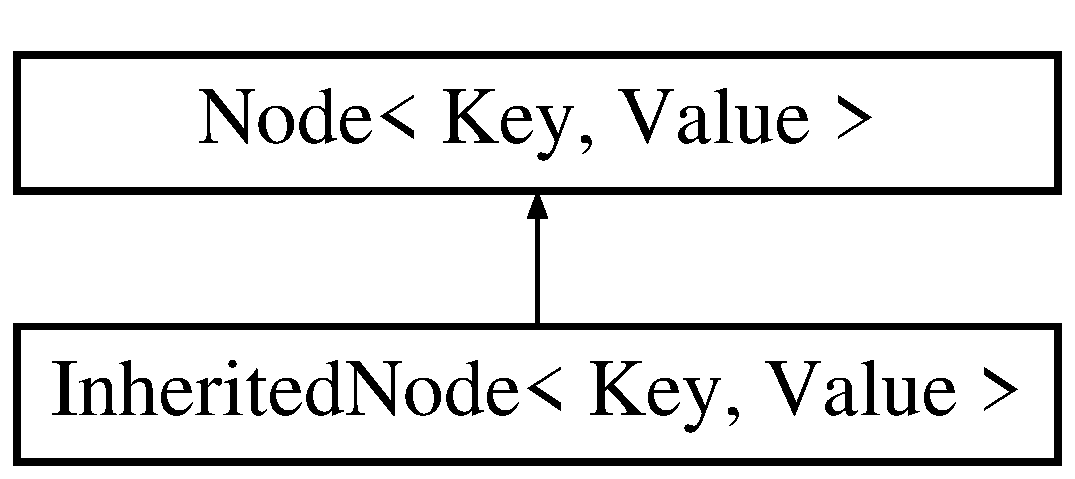
\includegraphics[height=2.000000cm]{classNode}
\end{center}
\end{figure}
\subsection*{Public Member Functions}
\begin{DoxyCompactItemize}
\item 
\mbox{\hyperlink{classNode_ac9bdc0036be15ac4b622696c804c501f}{Node}} (const Key \&key, const Value \&value, \mbox{\hyperlink{classNode}{Node}}$<$ Key, Value $>$ $\ast$parent)
\item 
virtual \mbox{\hyperlink{classNode_aaa753148a7bac7330974f1a9bc9249f1}{$\sim$\+Node}} ()
\item 
const std\+::pair$<$ const Key, Value $>$ \& \mbox{\hyperlink{classNode_a41e3bd64767b0a5ed30c6f9d8d6b3ead}{get\+Item}} () const
\item 
std\+::pair$<$ const Key, Value $>$ \& \mbox{\hyperlink{classNode_a4e683e6ac10c3015939f9598bb2c2629}{get\+Item}} ()
\item 
const Key \& \mbox{\hyperlink{classNode_a9ad1feabf07e276143802749d48a5736}{get\+Key}} () const
\item 
const Value \& \mbox{\hyperlink{classNode_a8c36066d5be674c07d2b3805cc76fc08}{get\+Value}} () const
\item 
Value \& \mbox{\hyperlink{classNode_abdbbc3b9627d1bfe2106c2000d410811}{get\+Value}} ()
\item 
virtual \mbox{\hyperlink{classNode}{Node}}$<$ Key, Value $>$ $\ast$ \mbox{\hyperlink{classNode_a69339fc2a76f5b4456ecc930703f93cd}{get\+Parent}} () const
\item 
virtual \mbox{\hyperlink{classNode}{Node}}$<$ Key, Value $>$ $\ast$ \mbox{\hyperlink{classNode_aaa2c1b8458c0df8489ac991cf03d3c33}{get\+Left}} () const
\item 
virtual \mbox{\hyperlink{classNode}{Node}}$<$ Key, Value $>$ $\ast$ \mbox{\hyperlink{classNode_a148e0ef6995e7c8aa344779e0cca507a}{get\+Right}} () const
\item 
int \mbox{\hyperlink{classNode_a42201a49f8c8bef979f79baa75d70109}{get\+Height}} () const
\item 
void \mbox{\hyperlink{classNode_a981799e30e7649812c2ad3a2d43c3f94}{set\+Parent}} (\mbox{\hyperlink{classNode}{Node}}$<$ Key, Value $>$ $\ast$parent)
\item 
void \mbox{\hyperlink{classNode_af0a4ecd342adca0c1db88f0811ad0068}{set\+Left}} (\mbox{\hyperlink{classNode}{Node}}$<$ Key, Value $>$ $\ast$left)
\item 
void \mbox{\hyperlink{classNode_ade5c16875afa559250c7a49d56007685}{set\+Right}} (\mbox{\hyperlink{classNode}{Node}}$<$ Key, Value $>$ $\ast$right)
\item 
void \mbox{\hyperlink{classNode_ab9b9a0da6a6b481623a3d1a7de5594a9}{set\+Value}} (const Value \&value)
\item 
void \mbox{\hyperlink{classNode_ada6fa2c6e9c7ab2330e63ab44199ed35}{set\+Height}} (int height)
\end{DoxyCompactItemize}
\subsection*{Protected Attributes}
\begin{DoxyCompactItemize}
\item 
\mbox{\Hypertarget{classNode_a7d5cce0902ef996ebf45451db8b667fb}\label{classNode_a7d5cce0902ef996ebf45451db8b667fb}} 
std\+::pair$<$ const Key, Value $>$ {\bfseries m\+Item}
\item 
\mbox{\Hypertarget{classNode_a0edda9f5ea45078bef125a1298de9bef}\label{classNode_a0edda9f5ea45078bef125a1298de9bef}} 
\mbox{\hyperlink{classNode}{Node}}$<$ Key, Value $>$ $\ast$ {\bfseries m\+Parent}
\item 
\mbox{\Hypertarget{classNode_a93b44cfd9f890e4ac24b84bb4c06b68d}\label{classNode_a93b44cfd9f890e4ac24b84bb4c06b68d}} 
\mbox{\hyperlink{classNode}{Node}}$<$ Key, Value $>$ $\ast$ {\bfseries m\+Left}
\item 
\mbox{\Hypertarget{classNode_a3698d0c83982838834bc2218b15d7013}\label{classNode_a3698d0c83982838834bc2218b15d7013}} 
\mbox{\hyperlink{classNode}{Node}}$<$ Key, Value $>$ $\ast$ {\bfseries m\+Right}
\item 
\mbox{\Hypertarget{classNode_a2ca4a790470adabeff9e94becee1e000}\label{classNode_a2ca4a790470adabeff9e94becee1e000}} 
int {\bfseries m\+Height}
\end{DoxyCompactItemize}


\subsection{Detailed Description}
\subsubsection*{template$<$typename Key, typename Value$>$\newline
class Node$<$ Key, Value $>$}

A templated class for a \mbox{\hyperlink{classNode}{Node}} in a search tree. The getters for parent/left/right are virtual so that they can be overridden for future kinds of search trees, such as Red Black trees, Splay trees, and A\+VL trees. 

\subsection{Constructor \& Destructor Documentation}
\mbox{\Hypertarget{classNode_ac9bdc0036be15ac4b622696c804c501f}\label{classNode_ac9bdc0036be15ac4b622696c804c501f}} 
\index{Node@{Node}!Node@{Node}}
\index{Node@{Node}!Node@{Node}}
\subsubsection{\texorpdfstring{Node()}{Node()}}
{\footnotesize\ttfamily template$<$typename Key , typename Value $>$ \\
\mbox{\hyperlink{classNode}{Node}}$<$ Key, Value $>$\+::\mbox{\hyperlink{classNode}{Node}} (\begin{DoxyParamCaption}\item[{const Key \&}]{key,  }\item[{const Value \&}]{value,  }\item[{\mbox{\hyperlink{classNode}{Node}}$<$ Key, Value $>$ $\ast$}]{parent }\end{DoxyParamCaption})}

Explicit constructor for a node. \mbox{\Hypertarget{classNode_aaa753148a7bac7330974f1a9bc9249f1}\label{classNode_aaa753148a7bac7330974f1a9bc9249f1}} 
\index{Node@{Node}!````~Node@{$\sim$\+Node}}
\index{````~Node@{$\sim$\+Node}!Node@{Node}}
\subsubsection{\texorpdfstring{$\sim$\+Node()}{~Node()}}
{\footnotesize\ttfamily template$<$typename Key , typename Value $>$ \\
\mbox{\hyperlink{classNode}{Node}}$<$ Key, Value $>$\+::$\sim$\mbox{\hyperlink{classNode}{Node}} (\begin{DoxyParamCaption}{ }\end{DoxyParamCaption})\hspace{0.3cm}{\ttfamily [virtual]}}

Destructor, which does not need to do anything since the pointers inside of a node are only used as references to existing nodes. The nodes pointed to by parent/left/right are freed within the delete\+All() helper method in the \mbox{\hyperlink{classBinarySearchTree}{Binary\+Search\+Tree}}. 

\subsection{Member Function Documentation}
\mbox{\Hypertarget{classNode_a42201a49f8c8bef979f79baa75d70109}\label{classNode_a42201a49f8c8bef979f79baa75d70109}} 
\index{Node@{Node}!get\+Height@{get\+Height}}
\index{get\+Height@{get\+Height}!Node@{Node}}
\subsubsection{\texorpdfstring{get\+Height()}{getHeight()}}
{\footnotesize\ttfamily template$<$typename Key , typename Value $>$ \\
int \mbox{\hyperlink{classNode}{Node}}$<$ Key, Value $>$\+::get\+Height (\begin{DoxyParamCaption}{ }\end{DoxyParamCaption}) const}

A const getter for the height. \mbox{\Hypertarget{classNode_a41e3bd64767b0a5ed30c6f9d8d6b3ead}\label{classNode_a41e3bd64767b0a5ed30c6f9d8d6b3ead}} 
\index{Node@{Node}!get\+Item@{get\+Item}}
\index{get\+Item@{get\+Item}!Node@{Node}}
\subsubsection{\texorpdfstring{get\+Item()}{getItem()}\hspace{0.1cm}{\footnotesize\ttfamily [1/2]}}
{\footnotesize\ttfamily template$<$typename Key , typename Value $>$ \\
const std\+::pair$<$ const Key, Value $>$ \& \mbox{\hyperlink{classNode}{Node}}$<$ Key, Value $>$\+::get\+Item (\begin{DoxyParamCaption}{ }\end{DoxyParamCaption}) const}

A const getter for the item. \mbox{\Hypertarget{classNode_a4e683e6ac10c3015939f9598bb2c2629}\label{classNode_a4e683e6ac10c3015939f9598bb2c2629}} 
\index{Node@{Node}!get\+Item@{get\+Item}}
\index{get\+Item@{get\+Item}!Node@{Node}}
\subsubsection{\texorpdfstring{get\+Item()}{getItem()}\hspace{0.1cm}{\footnotesize\ttfamily [2/2]}}
{\footnotesize\ttfamily template$<$typename Key , typename Value $>$ \\
std\+::pair$<$ const Key, Value $>$ \& \mbox{\hyperlink{classNode}{Node}}$<$ Key, Value $>$\+::get\+Item (\begin{DoxyParamCaption}{ }\end{DoxyParamCaption})}

A non-\/const getter for the item. \mbox{\Hypertarget{classNode_a9ad1feabf07e276143802749d48a5736}\label{classNode_a9ad1feabf07e276143802749d48a5736}} 
\index{Node@{Node}!get\+Key@{get\+Key}}
\index{get\+Key@{get\+Key}!Node@{Node}}
\subsubsection{\texorpdfstring{get\+Key()}{getKey()}}
{\footnotesize\ttfamily template$<$typename Key , typename Value $>$ \\
const Key \& \mbox{\hyperlink{classNode}{Node}}$<$ Key, Value $>$\+::get\+Key (\begin{DoxyParamCaption}{ }\end{DoxyParamCaption}) const}

A const getter for the key. \mbox{\Hypertarget{classNode_aaa2c1b8458c0df8489ac991cf03d3c33}\label{classNode_aaa2c1b8458c0df8489ac991cf03d3c33}} 
\index{Node@{Node}!get\+Left@{get\+Left}}
\index{get\+Left@{get\+Left}!Node@{Node}}
\subsubsection{\texorpdfstring{get\+Left()}{getLeft()}}
{\footnotesize\ttfamily template$<$typename Key , typename Value $>$ \\
\mbox{\hyperlink{classNode}{Node}}$<$ Key, Value $>$ $\ast$ \mbox{\hyperlink{classNode}{Node}}$<$ Key, Value $>$\+::get\+Left (\begin{DoxyParamCaption}{ }\end{DoxyParamCaption}) const\hspace{0.3cm}{\ttfamily [virtual]}}

An implementation of the virtual function for retreiving the left child. \mbox{\Hypertarget{classNode_a69339fc2a76f5b4456ecc930703f93cd}\label{classNode_a69339fc2a76f5b4456ecc930703f93cd}} 
\index{Node@{Node}!get\+Parent@{get\+Parent}}
\index{get\+Parent@{get\+Parent}!Node@{Node}}
\subsubsection{\texorpdfstring{get\+Parent()}{getParent()}}
{\footnotesize\ttfamily template$<$typename Key , typename Value $>$ \\
\mbox{\hyperlink{classNode}{Node}}$<$ Key, Value $>$ $\ast$ \mbox{\hyperlink{classNode}{Node}}$<$ Key, Value $>$\+::get\+Parent (\begin{DoxyParamCaption}{ }\end{DoxyParamCaption}) const\hspace{0.3cm}{\ttfamily [virtual]}}

An implementation of the virtual function for retreiving the parent. \mbox{\Hypertarget{classNode_a148e0ef6995e7c8aa344779e0cca507a}\label{classNode_a148e0ef6995e7c8aa344779e0cca507a}} 
\index{Node@{Node}!get\+Right@{get\+Right}}
\index{get\+Right@{get\+Right}!Node@{Node}}
\subsubsection{\texorpdfstring{get\+Right()}{getRight()}}
{\footnotesize\ttfamily template$<$typename Key , typename Value $>$ \\
\mbox{\hyperlink{classNode}{Node}}$<$ Key, Value $>$ $\ast$ \mbox{\hyperlink{classNode}{Node}}$<$ Key, Value $>$\+::get\+Right (\begin{DoxyParamCaption}{ }\end{DoxyParamCaption}) const\hspace{0.3cm}{\ttfamily [virtual]}}

An implementation of the virtual function for retreiving the right child. \mbox{\Hypertarget{classNode_a8c36066d5be674c07d2b3805cc76fc08}\label{classNode_a8c36066d5be674c07d2b3805cc76fc08}} 
\index{Node@{Node}!get\+Value@{get\+Value}}
\index{get\+Value@{get\+Value}!Node@{Node}}
\subsubsection{\texorpdfstring{get\+Value()}{getValue()}\hspace{0.1cm}{\footnotesize\ttfamily [1/2]}}
{\footnotesize\ttfamily template$<$typename Key , typename Value $>$ \\
const Value \& \mbox{\hyperlink{classNode}{Node}}$<$ Key, Value $>$\+::get\+Value (\begin{DoxyParamCaption}{ }\end{DoxyParamCaption}) const}

A const getter for the value. \mbox{\Hypertarget{classNode_abdbbc3b9627d1bfe2106c2000d410811}\label{classNode_abdbbc3b9627d1bfe2106c2000d410811}} 
\index{Node@{Node}!get\+Value@{get\+Value}}
\index{get\+Value@{get\+Value}!Node@{Node}}
\subsubsection{\texorpdfstring{get\+Value()}{getValue()}\hspace{0.1cm}{\footnotesize\ttfamily [2/2]}}
{\footnotesize\ttfamily template$<$typename Key , typename Value $>$ \\
Value \& \mbox{\hyperlink{classNode}{Node}}$<$ Key, Value $>$\+::get\+Value (\begin{DoxyParamCaption}{ }\end{DoxyParamCaption})}

A non-\/const getter for the value. \mbox{\Hypertarget{classNode_ada6fa2c6e9c7ab2330e63ab44199ed35}\label{classNode_ada6fa2c6e9c7ab2330e63ab44199ed35}} 
\index{Node@{Node}!set\+Height@{set\+Height}}
\index{set\+Height@{set\+Height}!Node@{Node}}
\subsubsection{\texorpdfstring{set\+Height()}{setHeight()}}
{\footnotesize\ttfamily template$<$typename Key , typename Value $>$ \\
void \mbox{\hyperlink{classNode}{Node}}$<$ Key, Value $>$\+::set\+Height (\begin{DoxyParamCaption}\item[{int}]{height }\end{DoxyParamCaption})}

A setter for the height of a node. \mbox{\Hypertarget{classNode_af0a4ecd342adca0c1db88f0811ad0068}\label{classNode_af0a4ecd342adca0c1db88f0811ad0068}} 
\index{Node@{Node}!set\+Left@{set\+Left}}
\index{set\+Left@{set\+Left}!Node@{Node}}
\subsubsection{\texorpdfstring{set\+Left()}{setLeft()}}
{\footnotesize\ttfamily template$<$typename Key , typename Value $>$ \\
void \mbox{\hyperlink{classNode}{Node}}$<$ Key, Value $>$\+::set\+Left (\begin{DoxyParamCaption}\item[{\mbox{\hyperlink{classNode}{Node}}$<$ Key, Value $>$ $\ast$}]{left }\end{DoxyParamCaption})}

A setter for setting the left child of a node. \mbox{\Hypertarget{classNode_a981799e30e7649812c2ad3a2d43c3f94}\label{classNode_a981799e30e7649812c2ad3a2d43c3f94}} 
\index{Node@{Node}!set\+Parent@{set\+Parent}}
\index{set\+Parent@{set\+Parent}!Node@{Node}}
\subsubsection{\texorpdfstring{set\+Parent()}{setParent()}}
{\footnotesize\ttfamily template$<$typename Key , typename Value $>$ \\
void \mbox{\hyperlink{classNode}{Node}}$<$ Key, Value $>$\+::set\+Parent (\begin{DoxyParamCaption}\item[{\mbox{\hyperlink{classNode}{Node}}$<$ Key, Value $>$ $\ast$}]{parent }\end{DoxyParamCaption})}

A setter for setting the parent of a node. \mbox{\Hypertarget{classNode_ade5c16875afa559250c7a49d56007685}\label{classNode_ade5c16875afa559250c7a49d56007685}} 
\index{Node@{Node}!set\+Right@{set\+Right}}
\index{set\+Right@{set\+Right}!Node@{Node}}
\subsubsection{\texorpdfstring{set\+Right()}{setRight()}}
{\footnotesize\ttfamily template$<$typename Key , typename Value $>$ \\
void \mbox{\hyperlink{classNode}{Node}}$<$ Key, Value $>$\+::set\+Right (\begin{DoxyParamCaption}\item[{\mbox{\hyperlink{classNode}{Node}}$<$ Key, Value $>$ $\ast$}]{right }\end{DoxyParamCaption})}

A setter for setting the right child of a node. \mbox{\Hypertarget{classNode_ab9b9a0da6a6b481623a3d1a7de5594a9}\label{classNode_ab9b9a0da6a6b481623a3d1a7de5594a9}} 
\index{Node@{Node}!set\+Value@{set\+Value}}
\index{set\+Value@{set\+Value}!Node@{Node}}
\subsubsection{\texorpdfstring{set\+Value()}{setValue()}}
{\footnotesize\ttfamily template$<$typename Key , typename Value $>$ \\
void \mbox{\hyperlink{classNode}{Node}}$<$ Key, Value $>$\+::set\+Value (\begin{DoxyParamCaption}\item[{const Value \&}]{value }\end{DoxyParamCaption})}

A setter for the value of a node. 

The documentation for this class was generated from the following file\+:\begin{DoxyCompactItemize}
\item 
hw7\+\_\+provided\+\_\+bst.\+h\end{DoxyCompactItemize}

\hypertarget{classRotateTest}{}\section{Rotate\+Test Class Reference}
\label{classRotateTest}\index{Rotate\+Test@{Rotate\+Test}}
Inheritance diagram for Rotate\+Test\+:\begin{figure}[H]
\begin{center}
\leavevmode
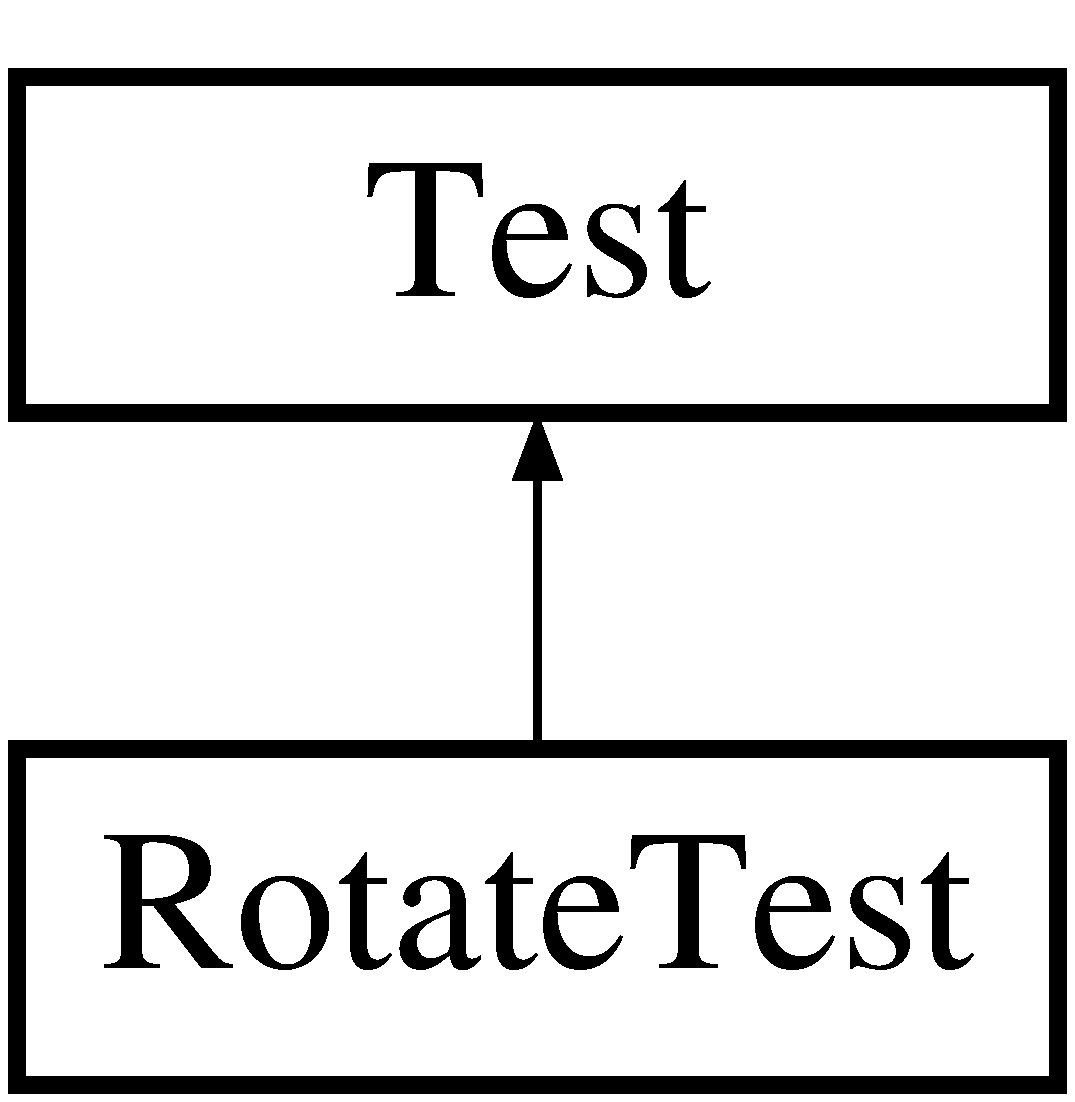
\includegraphics[height=2.000000cm]{classRotateTest}
\end{center}
\end{figure}
\subsection*{Protected Member Functions}
\begin{DoxyCompactItemize}
\item 
\mbox{\Hypertarget{classRotateTest_abf79269986c4d0167a7012c5d6a06334}\label{classRotateTest_abf79269986c4d0167a7012c5d6a06334}} 
void {\bfseries simple\+Tree\+Check} (\mbox{\hyperlink{classNode}{Node}}$<$ int, double $>$ $\ast$root)
\item 
\mbox{\Hypertarget{classRotateTest_a1dd78b04588e2773d0c607d91593a9dd}\label{classRotateTest_a1dd78b04588e2773d0c607d91593a9dd}} 
void {\bfseries stress\+Test\+Transform} (size\+\_\+t size, uint seed)
\item 
\mbox{\Hypertarget{classRotateTest_aad9a3080c84acf121fde68d2392653b4}\label{classRotateTest_aad9a3080c84acf121fde68d2392653b4}} 
void {\bfseries redirect\+Output} (std\+::ostream \&output, void($\ast$f)(const \mbox{\hyperlink{classInheritedRotate}{Stress\+Tree\+Type}} \&), const \mbox{\hyperlink{classInheritedRotate}{Stress\+Tree\+Type}} \&t)
\end{DoxyCompactItemize}


The documentation for this class was generated from the following file\+:\begin{DoxyCompactItemize}
\item 
hw7\+\_\+rotate\+\_\+test.\+cpp\end{DoxyCompactItemize}

%--- End generated contents ---

% Index
\backmatter
\newpage
\phantomsection
\clearemptydoublepage
\addcontentsline{toc}{chapter}{Index}
\printindex

\end{document}
